% ================================================================
% The Retrieve and Connect version of latex/starters/targeted/KS3/algebra/expandingBracketsStarter_workedSolutions.tex
%
% This is the same deck as the one above, made by renaming the titles in it.
% Every slide that was a numbered starter is now titled
% "Retrieve and Connect", and the word is renamed wherever else a title
% used it. Nothing outside a title has been changed.
%
%   made from           latex/starters/targeted/KS3/algebra/expandingBracketsStarter_workedSolutions.tex
%   retitling rules     version 1
%
% Please don't edit this file. It is written again from the one it was
% made from whenever that changes, so an edit here would be lost - edit
% that file instead and this one follows.
% ================================================================
% Root file used ashow macros
\documentclass{beamer}

% Theme (optional but nice)
\usetheme{Madrid}

% Maths
\usepackage{amsmath}

% Graphics
\usepackage{tikz}

% ================================================================
% Answer-overlay helpers
% ================================================================
\newcommand{\ablank}[1]{%
  \alt<2>{\textcolor{red}{#1}}{\underline{\phantom{#1}}}%
}
\newcommand{\ashow}[1]{\uncover<2->{\textcolor{red}{\small #1}}}
\newcommand{\ashowq}[1]{\alt<2->{\textcolor{red}{\small #1}}{?}}

% Answers drawn straight on to a TikZ diagram, revealed on overlay 2 like \ashow.
% Space is reserved on overlay 1, so the diagram does not move between slides.
\usetikzlibrary{overlay-beamer-styles}
\tikzset{
  ans/.style     = {red, thick, visible on=<2->},
  ansfill/.style = {red!15, visible on=<2->},
  anslab/.style  = {red, font=\tiny, visible on=<2->},
}

\title{Worked Solutions}
\author{Mathematics}
\date{}

\begin{document}

\frame{\titlepage}

\begin{frame}{Contents}
\small
\begin{columns}[T]
\begin{column}{0.48\textwidth}
\textbf{Questions and short answers}
\begin{itemize}
  \item \hyperlink{q-st1}{\beamergotobutton{Retrieve and Connect 1}}
\end{itemize}
\end{column}
\begin{column}{0.48\textwidth}
\textbf{Worked solutions}
\begin{itemize}
  \item \hyperlink{work-st1}{\beamergotobutton{Retrieve and Connect 1}}
\end{itemize}
\end{column}
\end{columns}
\end{frame}

% ---------- STARTER (PRIOR KNOWLEDGE) ----------
\begin{frame}{Retrieve and Connect}
\hypertarget{q-st1}{}
\begin{minipage}[t]{0.48\textwidth}

\begin{block}{1) Arithmetic}
\Large
\[
13 + 9 = \ablank{22}
\]
\end{block}

\vspace{6.2em}

\begin{block}{3) Collect like terms}
\Large
\[
3b + 4 + 2b = \ablank{5b+4}
\]
\end{block}

\end{minipage}\hfill
\begin{minipage}[t]{0.48\textwidth}

\begin{block}{2) Box Method}
\centering
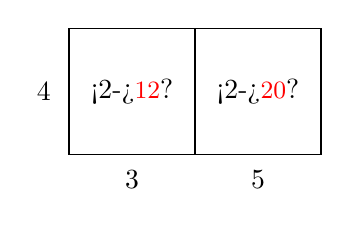
\begin{tikzpicture}[scale=0.8]

\draw (0,0) rectangle (4,2);
\draw (2,0) -- (2,2);

\node at (1,-0.4) {$3$};
\node at (3,-0.4) {$5$};
\node at (-0.4,1) {$4$};

\node at (1,1) {\ashowq{12}};
\node at (3,1) {\ashowq{20}};

\end{tikzpicture}

\vspace{0.4em}
Find the total area. \ashow{Total area $= 32$}

\end{block}

\vspace{0.6em}

\begin{block}{4) Expand the bracket}
\Large
\[
2(x+6) = \ablank{2x+12}
\]
\end{block}

\end{minipage}
\end{frame}

% ---------- WORKED SOLUTIONS FOR STARTER 1 ----------
\begin{frame}{Worked Solution: Retrieve and Connect 1, Question 1}
\hypertarget{work-st1}{}
\textbf{Question:} Calculate \(13+9\).

\uncover<2->{\textbf{Worked Solution:}
Use \(13=10+3\), so
\[
13+9 = 10+(3+9) = 10+12 = \ablank{22}.
\]}
\end{frame}

\begin{frame}{Worked Solution: Retrieve and Connect 1, Question 2}
\textbf{Question:} Use the box method to find the total area of the rectangle below.

\begin{center}
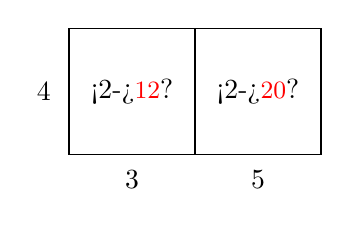
\begin{tikzpicture}[scale=0.8]
\draw (0,0) rectangle (4,2);
\draw (2,0) -- (2,2);

\node at (1,-0.4) {$3$};
\node at (3,-0.4) {$5$};
\node at (-0.4,1) {$4$};

\node at (1,1) {\ashowq{12}};
\node at (3,1) {\ashowq{20}};
\end{tikzpicture}
\end{center}

\uncover<2->{\textbf{Worked Solution:}
The two rectangles have areas \(3\times4\) and \(5\times4\). Therefore
\[
3\times4+5\times4 = 12+20 = \ablank{32}.
\]}
\end{frame}

\begin{frame}{Worked Solution: Retrieve and Connect 1, Question 3}
\textbf{Question:} Collect like terms: \(3b+4+2b\).

\uncover<2->{\textbf{Worked Solution:}
Collect the \(b\) terms and keep the constant separate:
\[
3b+4+2b = (3b+2b)+4 = \ablank{5b+4}.
\]}
\end{frame}

\begin{frame}{Worked Solution: Retrieve and Connect 1, Question 4}
\textbf{Question:} Expand the bracket: \(2(x+6)\).

\uncover<2->{\textbf{Worked Solution:}
Using the distributive property \(a(b+c)=ab+ac\),
\[
2(x+6) = 2\cdot x + 2\cdot 6 = \ablank{2x+12}.
\]}
\end{frame}

\end{document}